\chapter{Wyniki symulacji}
\section{Wyniki i statystyki}
Dzięki przyjętemu modelowi aplikacji łatwe jest zasymulowanie zewnętrznych sił działających na agenta. Widoczne jest to zwłaszcza w miejscach tzw. "wąskiego gardła".

\begin{figure}[h]
\centering
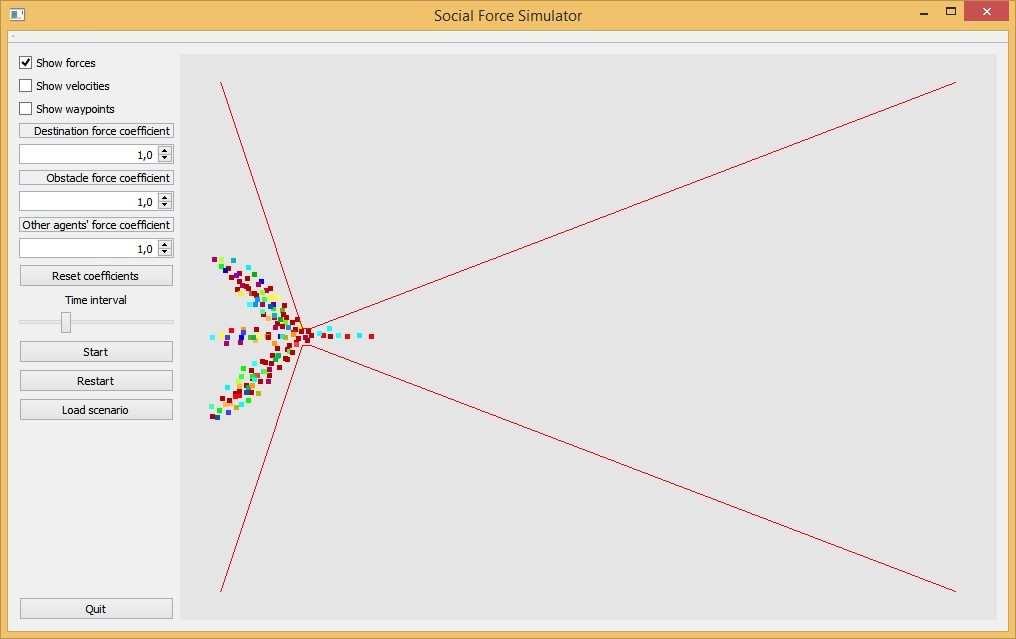
\includegraphics[scale=0.4]{waskie_gardlo_przyklad}
\caption{Wąskie gardło}
\end{figure}

Dane symulacji umożliwiają wykonania różnego rodzaju wykresów np. zmiany położenia pieszych, zmiany prędkości, zmiany sił działających na pieszego w czasie. 

\begin{figure}[h]
\centering
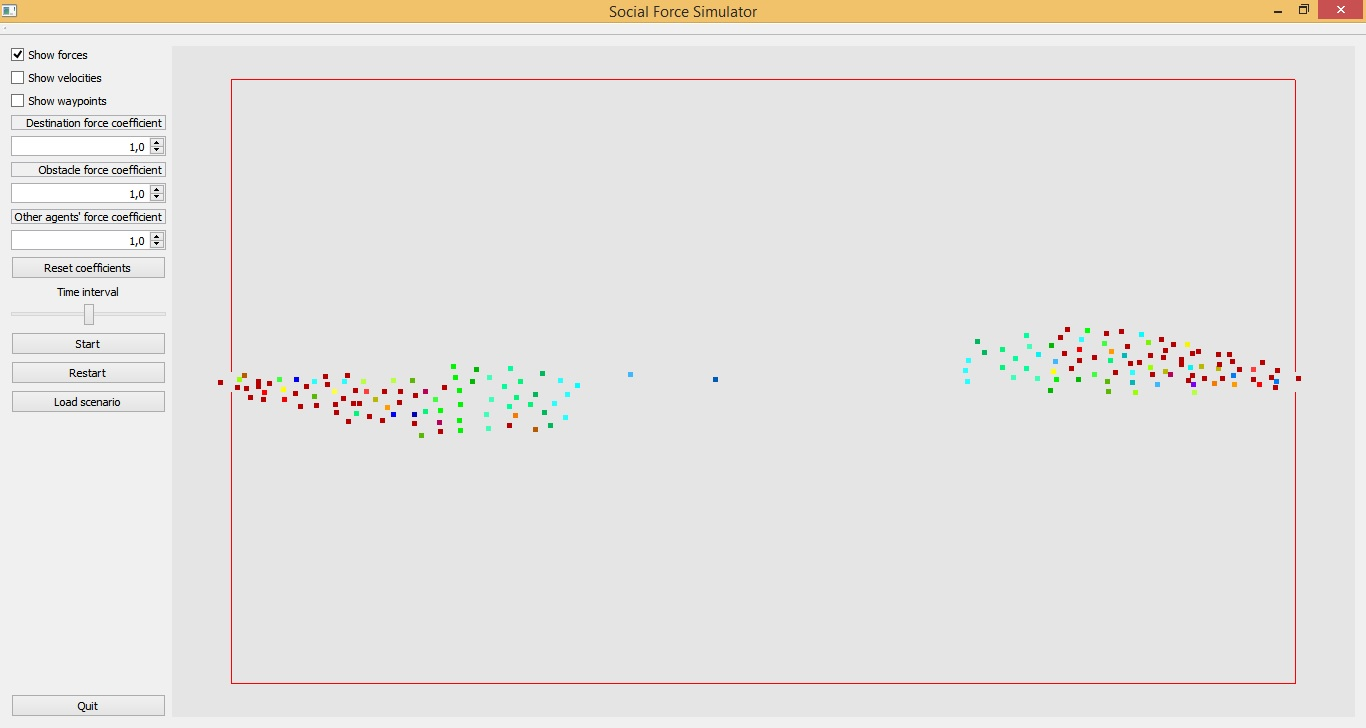
\includegraphics[scale=0.4]{przyklad_sil_dzialajacych_przy_waskim_gardle}
\caption{Przykład sił działających przy wąskim gardle}
\end{figure}

\begin{figure}[h]
\centering
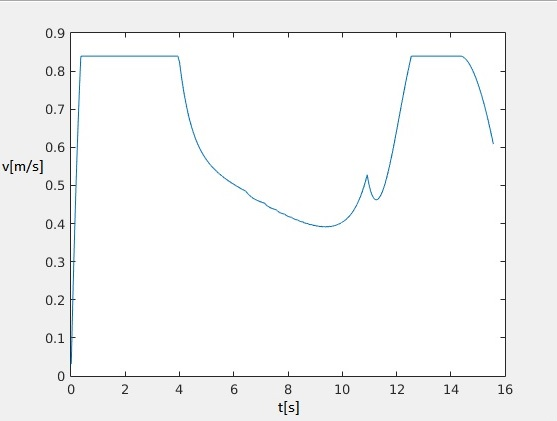
\includegraphics[scale=0.4]{wykres}
\caption{Wykres v(t) dla losowego aktora}
\end{figure}

Nagła jednostajna prędkość aktora spowodowana jest jest przyjęciem dla każdego aktora maksymalnej prędkości ograniczającej.
\newpage
\section{Zastosowane procedury kalibracji i walidacji}

Korzystając z uzyskanego modelu aplikacji staraliśmy się skalibrować parametry użyte w modelu ruchu pieszych, aby jak najwierniej odzwierciedlały rzeczywistość obserwowalną na co dzień.